
% Auriga theme
% https://github.com/anishathalye/auriga

\documentclass[14pt,aspectratio=169]{beamer}
\usepackage{pgfpages}
\usepackage{fancyvrb}
\usepackage{booktabs,dcolumn}
\usepackage{tikz}
\usetikzlibrary{arrows.meta, positioning, quotes}
\usepackage{pgfplots}

% \ifnotes
% \setbeamertemplate{note page}[plain]
% \setbeameroption{show notes on second screen=right}
% \fi

\usetheme{auriga}
\usecolortheme{auriga}

% define some colors for a consistent theme across slides
\definecolor{red}{RGB}{181, 23, 0}
\definecolor{blue}{RGB}{0, 118, 186}
\definecolor{gray}{RGB}{146, 146, 146}

\title{Historia Económica Argentina}

\author{\underline{Sebastián Freille} \inst{1}}

\institute[shortinst]{\inst{1} IEF-UNC \\ UCC}
\date{}

\AtBeginSection[]{
    \begin{frame}
    \vfill
    \centering
    \begin{beamercolorbox}[sep=8pt,center,shadow=true,rounded=true]{title}
        \usebeamerfont{title}\insertsectionhead\par%
    \end{beamercolorbox}
    \vfill
    \end{frame}
}



\AtBeginSubsection[]{
    \begin{frame}
    \vfill
    \centering
    \begin{beamercolorbox}[sep=6pt,center,shadow=true,rounded=true]{title}
        \usebeamerfont{title}\insertsubsectionhead\par%
    \end{beamercolorbox}
    \vfill
    \end{frame}
}


\AtBeginSubsubsection[]{
    \begin{frame}
    \vfill
    \centering
    \begin{beamercolorbox}[sep=4pt,center,shadow=true,rounded=true]{title}
        \usebeamerfont{title}\insertsubsubsectionhead\par%
    \end{beamercolorbox}
    \vfill
    \end{frame}
}


\begin{document}

{
  % rather than use the frame options [noframenumbering,plain], we make the
  % color match, so that the indicated page numbers match PDF page numbers
  \setbeamercolor{page number in head/foot}{fg=background canvas.bg}
  \begin{frame}
    \titlepage
  \end{frame}
}


\section{El Gobierno de Frondizi}

\begin{frame}\frametitle{La estrategia desarrollista}
                 \begin{itemize}\itemsep 5pt \medskip
                 \item Las políticas económicas llevadas a cabo en el
                   período 1958-62 fueron parte de un programa de
                   desarrollo de
                   largo plazo $\longrightarrow$ objetivo ambicioso de
                   producir cambios significativos y duradores en la
                   economía
                   \item Los principales ejes del programa del nuevo
                     presidente Frondizi fueron dos: 1) plan/programa
                     desarrollista; 2) plan de estabilización 
                   \end{itemize}
               \end{frame}


               
\begin{frame}\frametitle{La estrategia desarrollista (cont.)}
                 \begin{block}{¿Qué es el desarrollismo?}
El desarrollismo no fue una teoría económica sino más bien una estrategia
nacional de desarrollo. En los años 40, 50 y 60, tanto desarrollistas
como keynesianos dominaban el panorma económico de América Latina:
eran el \textit{mainstream}.  Partía de un diagnóstico aplicable a toda
región del mundo que no había completado su industrialización. Varios
postulados: 1) pesimismo respecto a exportaciones de productos
primarios (tesis Prebisch); 2) el desarrollo implicaba el desarrollo y
psao definitivo de una estructura agroexportadora a una completamente industrial
\end{block}
                 \end{frame}
               


\begin{frame}\frametitle{La estrategia desarrollista (cont.)}
                 \begin{block}{Visión de Rogelio Frigerio}
Visualiza la estructura económica argentina como subdesarrollada
``fruto de cien años de colonialismo''. Define al ``enemigo'' como a
fuerzas que se oponen a profundos cambios y especifica como ``el
conjunto de intereses que se benefician en la medida en que prevalecen
entre nosotros las condiciones de país puramente agropecuario y de
incipiente desarrollo industiral proveedor de productos primarios e
importador de combustibles, maquinarias y materias primas
industriales''. Es necesaria una política económica de desarrollo e
integración, priorizando las \textit{industrias de base}, \textit{la
  energía} y \textit{las comunicaciones}. 
\end{block}
                 \end{frame}
                 


\begin{frame}\frametitle{La estrategia desarrollista (cont.)}
                 \begin{itemize}\itemsep 5pt \medskip
                 \item La estrategia principal en Argentina fue la de
                   acelerar el crecimiento a través de un auemnto de
                   la inversión concentrada en un puñado de sectores
                   intensiovs en capital y sustitutivos de
                   importaciones.
                   \item El éxito de este programa dependía
                     fuertemente en la creación de un entorno
                     favorable a la inversión --economía sin
                     inflación, movilidad de K sin restricciones y
                     fomento de sectores ocn potencial de cuasirentas
                   \end{itemize}
               \end{frame}



\begin{frame}\frametitle{La estrategia desarrollista (cont.)}
                 \begin{itemize}\itemsep 5pt \medskip
                 \item Es importante revisar el diagnóstico de las
                   nuevas autoridades $\longrightarrow$ a fines de los
                   50s Argentina no había completado su proceso de
                   transformación comenzado en los 20s/30s. Por ello,
                   perdía importancia en relación a otros países
                   \item El desarrollismo sostenía que Argentina
                     estaba al borde del proceso que promovería el
                     despegue definitivo --concentrar inversión en
                     \textit{industrias básicas} a través de incentivos a
                     capital extranjero.
                   \end{itemize}
               \end{frame}


\begin{frame}\frametitle{La estrategia desarrollista (cont.)}
                 \begin{itemize}\itemsep 5pt \medskip
                 \item Entre las industrias básicas se priorizaron las
                   de extracción de petróleo y gas; química y
                   petroquímica; acero; extracción de carbón y hierro;
                   industria automotriz.
                   \item Las primeras medidas adoptadas por el nuevo
                     gobierno sin embargo iban en la dirección
                     contraria --aumentos de salarios nominales (y
                     reales), controles de precios y de M y controles
                     de tarifas de servicios públicos
                     \item Esto era explicado por necesidades
                       políticas [Frondizi gana con muchos votos
                       peronistas]
                   \end{itemize}
               \end{frame}
               


               \begin{frame}\frametitle{La estrategia desarrollista (cont.)}
                 \begin{itemize}\itemsep 5pt \medskip
                 \item Pero como explicamos la severa crisis de BP y
                   la creciente inflación 
                   hizo necesario un viraje $\longrightarrow$ medidas
                   para estimular IED (contratos, incentivos,
                   concesiones). Sanción de Ley de Inversiones
                   Extranjeras que puso al capital extranjero en
                   igualdad de condiciones que el capital nacional
                   \item Muchas de estas medidas sin embargo chocaron
                     con la realidad de alta y crónica inflación
                     $\longrightarrow$ anuncio del programa de estabilización de
                     1959 con el FMI
                   \end{itemize}
               \end{frame}
               

          
 
  \begin{frame}\frametitle{La estrategia desarrollista (cont.)}
\begin{figure}[hxtbp]\vspace{0cm}
  \centering
  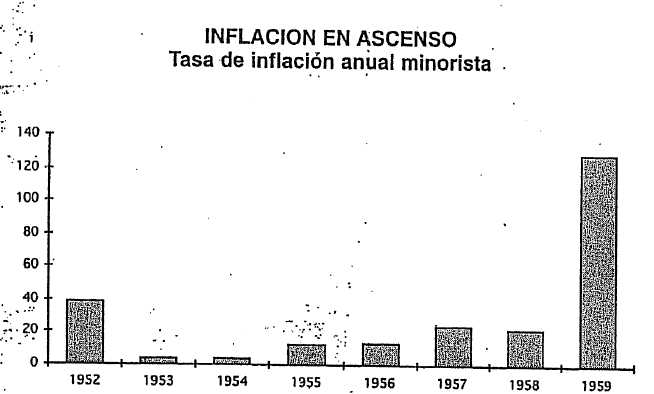
\includegraphics[scale=0.75]{uni4_des01}
   \label{fig:uni1_01}
\end{figure} 
  \end{frame}


  
               \begin{frame}\frametitle{La estrategia desarrollista (cont.)}
                 \begin{itemize}\itemsep 5pt \medskip
                 \item En diciembre de 1958 se anuncia un plan de
                   desarrollo y estabilización [Argentina se había
                   incorporado al FMI y BM en 1956] bajo la tutela del
                   FMI
                   \item El plan incluía --además de los clásicos
                     programas fiscales, monetarios y cambiarios- una
                     serie de medidas de liberalización internas y
                     externas.
                     \item Se eliminaron la gran mayoría de controles
                       de precios internos (con excepciones por
                       ejemplo alquileres urbanos) y se liberaron
                       tarifas de servicios públicos
                   \end{itemize}
               \end{frame}



               \begin{frame}\frametitle{La estrategia desarrollista (cont.)}
                 \begin{itemize}\itemsep 5pt \medskip
                 \item Luego de un primer año en que se aplicaron
                   medidas expansivas de estímulo a la demanda y de
                   protección de salarios y condiciones de vida,
                   Argentina se encamina a un programde fuerte ajuste
                   y desinflación
                   \item Se pasó de un sistema de controles cambiarios
                     con administración del TDC a un sistema de tipo
                     de cambio único y flexible --pero dados aranceles
                     a la M diferenciales, los TDC efectivos fueron
                     diferentes
                     \item Luego de varios meses se volvió a un tipo
                       de cambio fijo (con devaluación incluida)
                   \end{itemize}
               \end{frame}


               

\begin{frame}\frametitle{La estrategia desarrollista (cont.)}
\begin{figure}[hxtbp]\vspace{0cm}
  \centering
  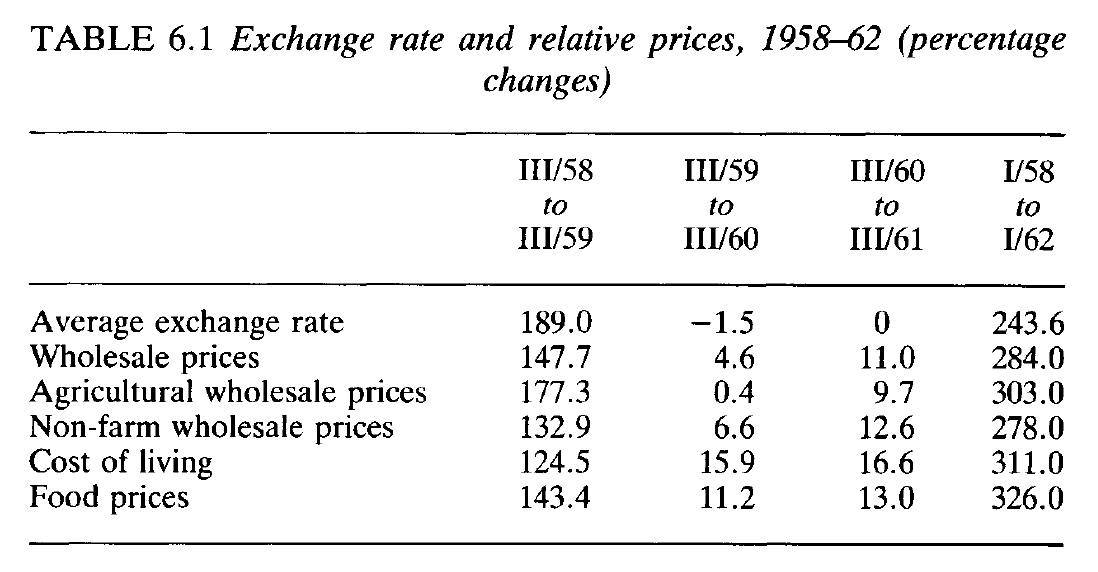
\includegraphics[scale=0.55]{uni4_des04}
   \label{fig:uni1_01}
\end{figure} 
\end{frame}


    \begin{frame}\frametitle{La estrategia desarrollista (cont.)}
                 \begin{itemize}\itemsep 5pt \medskip
                 \item El frente fiscal fue uno de los más dificiles
                   de resolver --aunque bajó fuertemente no se
                   eliminó.
                   \item Gran parte de la reducción vino por los
                     impuestos al comercio exterior
                     \item Las cuentas de gasto --tanto corriente como
                       de capital (inversión)- no variaron
                       significativamente.
                       \item La diferencia en la tabla puede ser
                         considerada como una aproximación del defícit fical
                   \end{itemize}
               \end{frame}



               
\begin{frame}\frametitle{La estrategia desarrollista (cont.)}
\begin{figure}[hxtbp]\vspace{0cm}
  \centering
  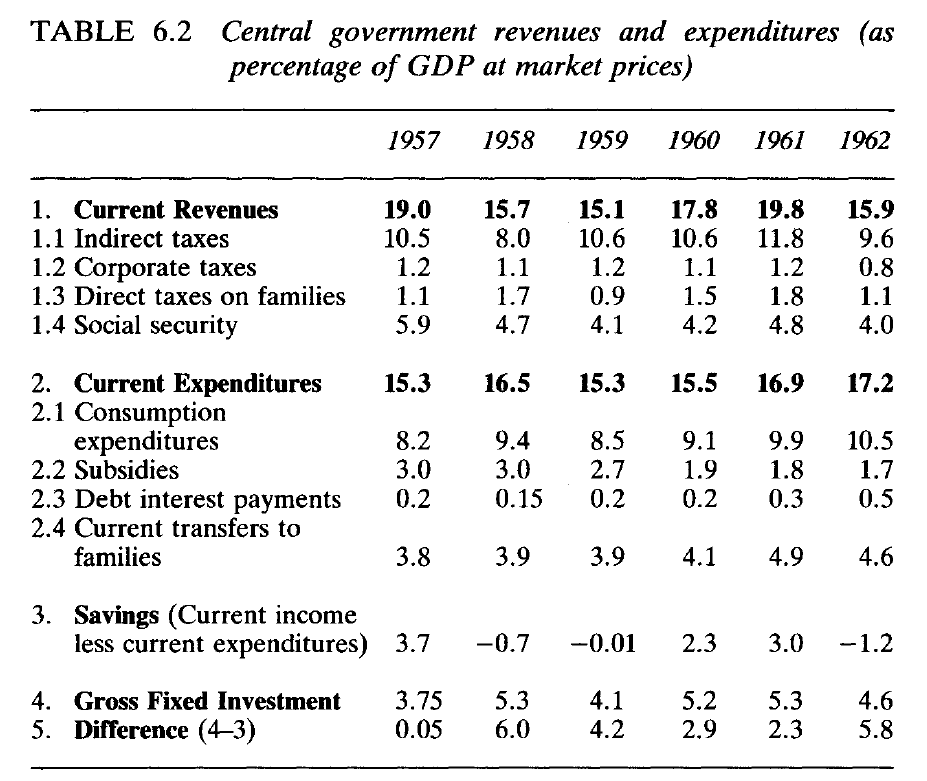
\includegraphics[scale=0.55]{uni4_des05}
   \label{fig:uni1_01}
\end{figure} 
\end{frame}



  \begin{frame}\frametitle{La estrategia desarrollista (cont.)}
                 \begin{itemize}\itemsep 5pt \medskip
                 \item La política monetaria tuvo un cambio importante
                   hacia 1960 $\longrightarrow$ mucho más restrictiva
                   --créditos del BCRA al sector público menores que
                   al sector privado
                   \item Esto fue consistente con una política
                     restrictiva de salarios --salarios nominales
                     pactados por convenio quedaron por abajo de
                     inflación
                     \item Los esfuerzos de estabilización y de
                       desarrollo afectaron la capacidad productiva y
                       su composición
                   \end{itemize}
               \end{frame}


 \begin{frame}\frametitle{La estrategia desarrollista (cont.)}
                 \begin{itemize}\itemsep 5pt \medskip
                 \item El PBI creció entre 1958 y 1961 aunque a tasa
                   moderada (3.6\% comparado con 1957). El aumento de
                   la absorción fue grande --10\% en el consumo pero
                   57\% en la inversión!
                   \item Sin embargo, grandes fluctuaciones hacia
                     adentro del período --picos en 1958 y 1962,
                     valles en 1959, recuperacion en 1960
                     \item Evaluación de desempeño macroeconómico
                       dificil dada la alta volatilidad --creció más
                       que durante los 1950s pero menos que en
                       1964-74. 
                   \end{itemize}
               \end{frame}


 \begin{frame}\frametitle{La situación del petróleo}
                 \begin{itemize}\itemsep 5pt \medskip
                 \item Una de las grandes ideas desarrollistas de la
                   época era que habia margen para sustituir
                   importaciones de petróleo
                   \item En 1958 gobierno anuncia firma de contratos
                     con empresas extranjeras $\longrightarrow$ muy
                     mala repercusión pública, gobierno a punto de
                     caer
                     \item Había acuerdo en en buscar una solución
                       para dejar de usar reservas para M de petróleo
                       $\longrightarrow$ algunos favorecían ampliar YPF
                     \item A pesar de todo, Frondizzi resistió y
                       pronto se verían los frutos
                   \end{itemize}
               \end{frame}



 \begin{frame}\frametitle{La situación del petróleo (cont.)}
                 \begin{itemize}\itemsep 5pt \medskip
                 \item Se triplicó la producción (de 5.5 a 16 millones
                   de m3) y se logró el autoabastecimiento
                   \item El escándalo de los contratos (sin licitación
                     ni aprobación legislativa) le costó el puesto a
                     Frigerio. Si bien en lo económico fue una medida
                     exitosa, Frondizzi perdió credibilidad y sobre
                     todo apoyo en los sectores nacionalistas
                     \item El tema del petróleo mostró hasta qué punto
                       Frondizzi estaba dispuesto a llevar a cabo su
                       programa desarrollista
                   \end{itemize}
               \end{frame}
               


 \begin{frame}\frametitle{Hacia el fin del programa}
                 \begin{itemize}\itemsep 5pt \medskip
                 \item Hacia 1961 se produce un cambio de ministros
                   (sale Alsogaray, entra Alemann) --situación externa
                   holgada y crecimiento interno pero dos problemas:
                   1) creciente déficit comercial; 2) presión sindical
                   por salarios
                    \item Rebrote de inflación en 1961 por ``empuje de
                      costos'' (política monetaria conservadora y
                      política fiscal sana)
                      \item El déficit sin embargo estaba reprimido
                        por la cuestión ferroviaria --larga puja que
                        terminó con el gobierno cediendo y pagando
                        altos costos
                   \end{itemize}
               \end{frame}



 \begin{frame}\frametitle{Hacia el fin del programa (cont.)}
                 \begin{itemize}\itemsep 5pt \medskip
                 \item El BCRA financió con emisión la ``solución''
                   ferroviaria y eso fue el golpe del muerte al plan
                   de estabilización
                   \item Al mismo tiempo, se corta el flujo de capital
                     hacia Argentina --con tipo de cambio fijo de
                     facto, esto implicaba salida de reservas y
                     consecuente restricción de liquidez y crédito
                     \item A fines de 1961, la devaluación aparecía
                       como inevitable --no sólo eso, en marzo de
                       1962, además de la devaluación, también cayó el gobierno
                   \end{itemize}
               \end{frame}
               
               

 \begin{frame}\frametitle{Dimensiones: Composición del producto}
                 \begin{itemize}\itemsep 5pt \medskip
                 \item La composición del producto muestra cambios
                   importantes dentro del sector manufacturero
                   --discontinuidad en desarrollo industrial
                   \item Desarrollo desparejo --actividades
                     priorizadas crecienron mucho, pero las mas
                     tradicionales crecieron poco y en algunos casos
                     menos que la población.
                     \item Gran creciimento de la mano de la industria
                       automotriz (tambien acero y plásticos)
                   \end{itemize}
               \end{frame}



                            
\begin{frame}\frametitle{Dimensiones: Composición del producto (cont.)}
\begin{figure}[hxtbp]\vspace{0cm}
  \centering
  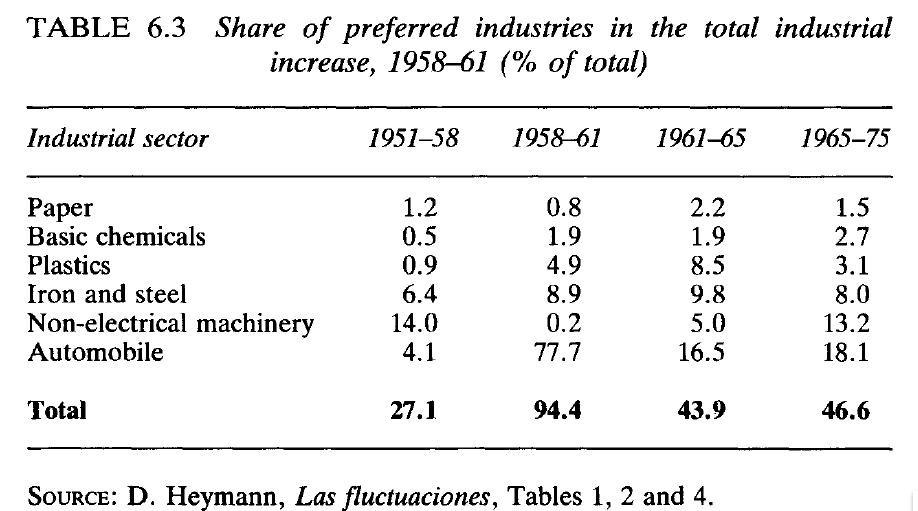
\includegraphics[scale=0.75]{uni4_des06}
   \label{fig:uni1_01}
\end{figure} 
\end{frame}


                          
\begin{frame}\frametitle{Dimensiones: Composición del producto (cont.)}
\begin{figure}[hxtbp]\vspace{0cm}
  \centering
  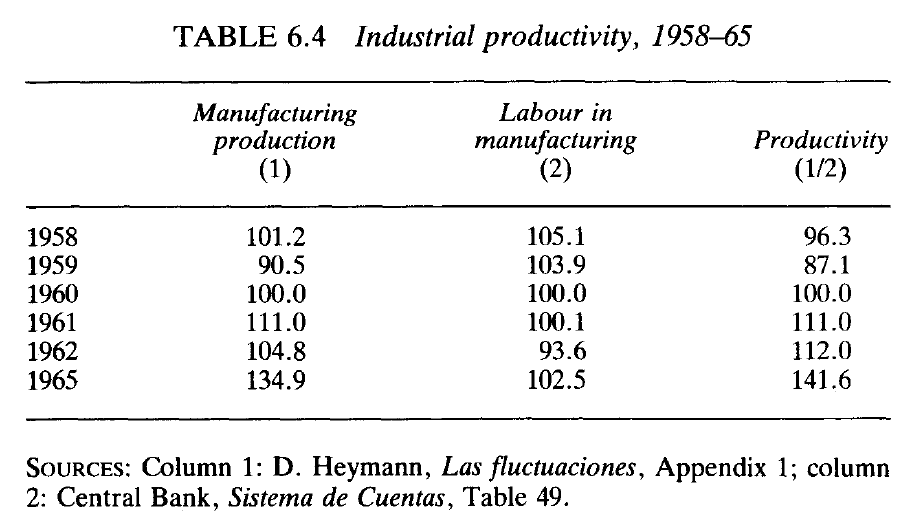
\includegraphics[scale=0.75]{uni4_des07}
   \label{fig:uni1_01}
\end{figure} 
\end{frame}




 \begin{frame}\frametitle{Dimensiones: Composición del producto (cont.)}
                 \begin{itemize}\itemsep 5pt \medskip
                 \item Fuertes incentivos también fueron a la
                   extracción de petróleo y gas --gran incremento en
                   producción al tiempo que se sustituian
                   M. 
                   \item Algo similar pero en menor medida pasó con la
                     producción e importación de carbón. 
\item Producción de petróleo se triplicó durante este periodo (M
  bajaron de 57 a 7\% de oferta total). 
                   \end{itemize}
               \end{frame}



                \begin{frame}\frametitle{Dimensiones: Balanza de pagos}
                 \begin{itemize}\itemsep 5pt \medskip
                 \item La balanza de pagos fue uno de los puntos más
                   débiles de la estrategia desarrolista del gobierno
                   --sólo en 1959 debido a la devaluación la balanza
                   comercial es positiva; luego deficitaria en
                   1960-62.
                   \item No hubo una contribución significativa de las
                     exportaciones a mejorar el balance comercial
                     --apenas la economía retomó el crecimiento, la
                     situación se volvió crítica (demanda de M para
                     industrias sobre todo no prioritarias; fuertes M
                     de bienes de capital y maquinarias
                   \end{itemize}
               \end{frame}



                  \begin{frame}\frametitle{Dimensiones: Balanza de
                      pagos (cont.)}
                 \begin{itemize}\itemsep 5pt \medskip
                 \item La cuenta capital tuvo saldos favorables en
                   general debido a la entrada de capital y IED
                   --empezó a revertirse con el deterioro del TCR por
                   aumento de $P_{NT}$ --hacia 1961 la pérdida de
                   reservas anticipaba futuras devaluaciones
                   \item Esto fue agravado por los aumentos de
                     servicios financieros (deuda) y las remesas de
                     utilidades de compañias extranjeras --mas presión
                     sobre la cuenta K del BP
                   \end{itemize}
               \end{frame}


  \begin{frame}\frametitle{Dimensiones: Salarios reales y distribución
      del Y}
                 \begin{itemize}\itemsep 5pt \medskip
                 \item Frondizi fue criticado por los efectos del
                   programa económico sobre la distribución del Y y
                   salarios reales --situación que venía por lo menos
                   desde 1955.
                   \item Entre 1953 y 1961 sólo deciles más altos
                     mejoraron su posición; los más bajos la
                     empeoraron
                     \item El año 1959 marca un quiebre --la recesión
                       de ese año empeoró mucho los salarios reales y
                       aunque recuperaron algo hacia 1961, no lograron
                       recuperarse a niveles previos
                   \end{itemize}
               \end{frame}


                        
\begin{frame}\frametitle{Dimensiones: Salarios reales y distribución
    del Y}
\begin{figure}[hxtbp]\vspace{0cm}
  \centering
  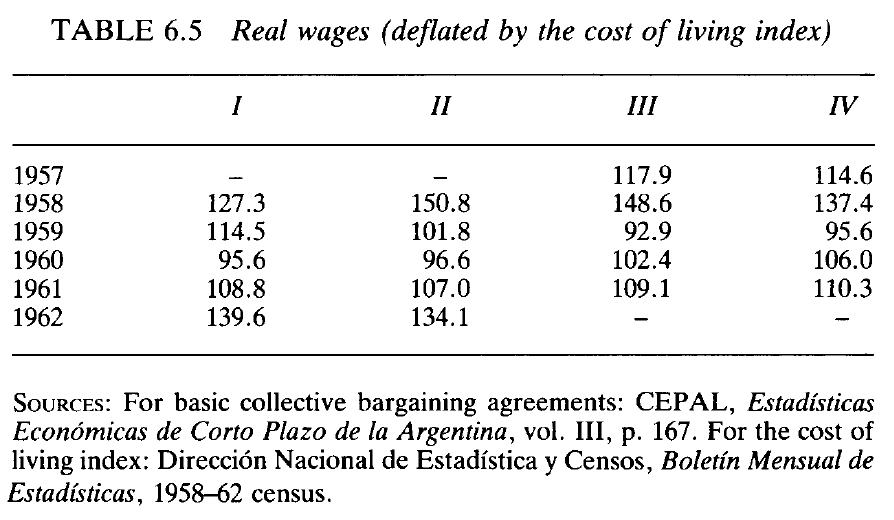
\includegraphics[scale=0.65]{uni4_des08}
   \label{fig:uni1_01}
\end{figure} 
\end{frame}




 \begin{frame}\frametitle{Dimensiones: Inflación}
                 \begin{itemize}\itemsep 5pt \medskip
                 \item Al principio la inflación aumentó debido a la
                   política expansiva (1958) --no obstante entre 1959
                   y 1961-62 los aumentos de precios fueron reducidos
                   significativamente.
                   \item Hubo bruscos movimientos de precios
                     relativos --precios de productos agropecuarois
                     aumentaron fuerte en 1958 y hasta 1959 para luego
                     ceder ante los precios de productos sustitutivos
                     de M de bienes no transables
                     \item Esto impactó naturalmente en el
                       estancamiento de X y la estrategia desarrolista
                   \end{itemize}
               \end{frame}


               


  
               
                 
               
\section{El interregno de 1962-63}


  \begin{frame}\frametitle{Transición y movimientos}
    \begin{itemize}\itemsep 10pt
    \item Guido (presidía el Senado) es designado por los militares
      pero el poder residía en ellos --¿pero quiénes eran las Fuerzas
      Armadas?
      \item Fuertes internas --legalistas/azules y colorados. La
        cuestión de fondo era la posición ante el peronismo y la
        relación con el poder
        \item Legalistas $\longrightarrow$ inevitable y deseable la
          vuelta a la constitucionalidad --colorados proponían una
          larga y permanente dictadura
        \end{itemize}
               \end{frame}



  \begin{frame}\frametitle{Transición y movimientos (cont.)}
    \begin{itemize}\itemsep 10pt
    \item La normalidad era el cambio continuo --en las personas y
      roles. Continuas idas y vueltas hacía difícil la convivencia
      \item A los seis meses, se produce la lucha armada y triunfa los
        azules (legalistas) --se reflotaba la esperanza de una retorno
        democrático
        \item Se fijan elecciones para julio de 1963 aunque aún con el
          peronismo proscripto.
          \item Arturo Illia (UCRP) gana con el 25\% de los votos (hubo 19\%
            de voto en blanco) --se abría paso a una nueva etapa
        \end{itemize}
               \end{frame}



  \begin{frame}\frametitle{El breve gobierno de Guido}
    \begin{itemize}\itemsep 10pt
    \item Guido devaluó la moneda más del 50\% para para la sangría de
      reservas. Prioridades eran contener déficit fiscal y la emisión
      monetaria
      \item La inflación continuó alta (parcialmente por efecto de la
        devaluación) y había un fuerte rechazo del peso
        \item Luego de mucho, la recesión de fines de
          1962-med 1963 pegó fuerte en el empleo (casi un 9\%)
          \item La recesión operó por el canal de crédito --al
            cortarse el crédito externo, también lo hizo el interno y
            las empresas contrajeron producción y vendieron stocks
        \end{itemize}
               \end{frame}


\begin{frame}\frametitle{El breve gobierno de Guido (cont.)}
    \begin{itemize}\itemsep 10pt
    \item No hubo mucho que Guido pudo hacer (tuvo 4 ministros de
      economía) más allá de buscar la ortodoxia en la política
      económica
      \item La situación de recesión con inflación se mantuvo durante
        su breve mandato --sumando contexto político y económico, tal
        vez hizo frente a una de las peores herencias
        \item Reequilibró en parte los precios relativos para ser más
          compatible con equilibrio externo pero quedaban desafíos
          --definir perfil productivo y el rol del Estado en la
          economía. Ese es el contexto en que asume Illia
        \end{itemize}
               \end{frame}
               


 \begin{frame}\frametitle{El breve gobierno de Guido (cont.)}
\begin{figure}[hxtbp]\vspace{0cm}
  \centering
  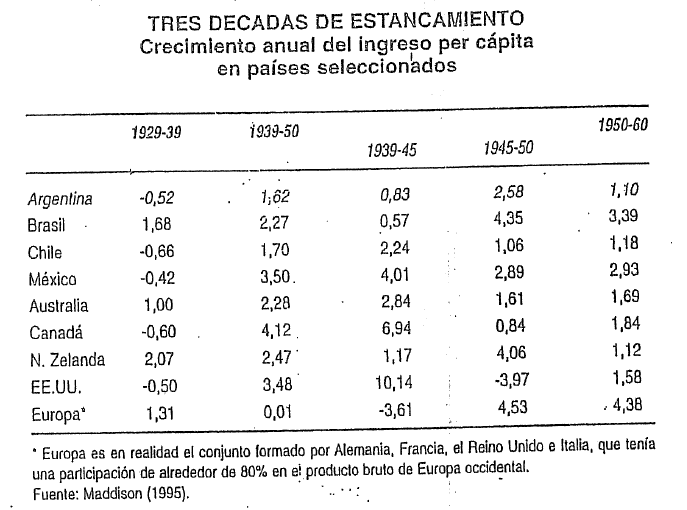
\includegraphics[scale=0.6]{uni4_indus03}
   \caption{Décadas de estancamiento}
\end{figure} 
  \end{frame}
               

               

  

\begin{frame}\frametitle{El breve gobierno de Guido (cont.)}
    \begin{itemize}\itemsep 10pt
    \item Argentina en 1950-60 fue
      el de peor crecimiento --tambien muy mal desempeño en la
      década infame.
      \item Evidente que modelo y crecimiento experimentado hasta
        1930 terminado para siempre --¿cuál era la alternativa?
        \item Desarrollismo fue creativ para impulsar una economía semi-industrializada y orientada al
          mdo interno
          \item A diferencia de la no-estrategia de LP de Perón, el
            desarrollismo si planteó una estrategia de LP --¿el fracaso fue sólo por la crisis de 1962? ¿hubo
            algún merito? ¿cómo explicar el crecimiento de 1963-73?
        \end{itemize}
               \end{frame}



                \section{Evaluación del desarrollismo}
  


               


               \begin{frame}\frametitle{El desarrollismo en
                   perspectiva}
    \begin{itemize}\itemsep 10pt
    \item Hipótesis sobre industrialización en América Latina
      \begin{itemize}\itemsep 5pt \medskip
      \item Hipótesis de ``shocks negativos'' [Singer (1950), Prebish (1950), Furtado
        (1959)] $\longrightarrow$ declinación de TIE y demanda interna
        de manufacturas es cubierta con producción local --hipótesis
        relacionada con \textit{enfermedad holandesa} ya que países se
        \textit{desindustrializan} con booms y
        \textit{reindustrializan} con TIE decrecientes
        \item Hipótesis de ``industrialización endógena'' [Dean
          (1969), Díaz-Alejandro (1976)] $\longrightarrow$
          industrialización surge con boom de exportaciones lo que
          facilita importar K --y via un efecto ingreso que permite
          mayor demanda de producción industrial
        \end{itemize}
                        \end{itemize}
               \end{frame}




               

 \begin{frame}\frametitle{El desarrollismo en perspectiva (cont.)}
    \begin{itemize}\itemsep 10pt
    \item Hipótesis sobre industrialización en América Latina (cont.)
      \begin{itemize}\itemsep 5pt \medskip
      \item Hipótesis de ISI $\longrightarrow$ política explícita de
        apoyo industrial incluyendo aranceles, controles cambiarios y
        preferencias por firmas locales [Baer (1972), Hirschmann (1968)]
        \item Hipótesis ISI ``estancamientista'' $\longrightarrow$ no
          proveía incentivos a aumentar productividad en el tiempo
          --ISI como fenómeno exitoso de corto/mediano plazo
          [Bulmer-Thomas (2003), Diaz-Alejandro (1970), Krueger (1978)]
        \end{itemize}
        \item Ninguna de estas hipótesis \textit{per se} puede
          explicar las experiencias diferenciales de los países de
          Latam --condiciones iniciales tan o más importantes que
          shocks negativos
                        \end{itemize}
               \end{frame}

               
               

 \begin{frame}\frametitle{El desarrollismo en perspectiva (cont.)}
\begin{figure}[hxtbp]\vspace{0cm}
  \centering
  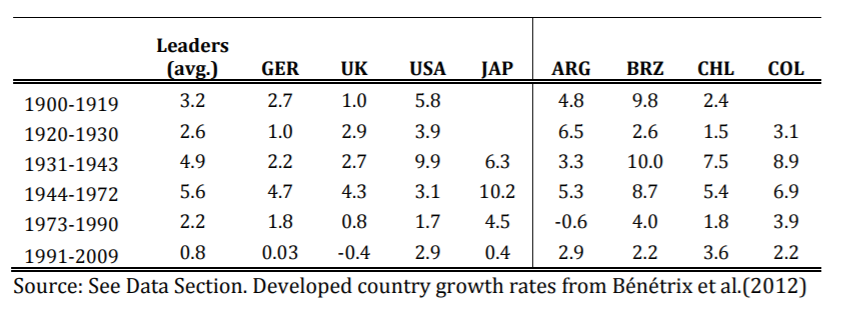
\includegraphics[scale=0.7]{uni4_indus01}
   \caption{Tasa de crecimiento del PBI industrial. Fuente: della
     Paolera et al (NBER, 2018)}
\end{figure} 
  \end{frame}
               


   \begin{frame}\frametitle{El desarrollismo en perspectiva (cont.)}
\begin{figure}[hxtbp]\vspace{0cm}
  \centering
  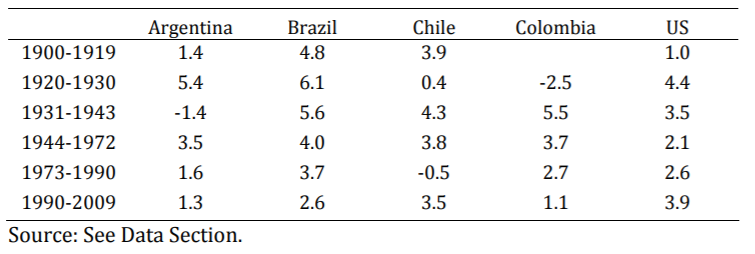
\includegraphics[scale=0.7]{uni4_indus02}
   \caption{Tasa de crecimiento productividad laboral media. Fuente: della
     Paolera et al (NBER, 2018)}
\end{figure} 
  \end{frame}
               


 \begin{frame}\frametitle{El desarrollismo en perspectiva}
    \begin{itemize}\itemsep 10pt
      \item El \textit{desarrollismo} en Argentina nunca logró el
        éxito que tuvo el \textit{desenvolvimentismo} de Kubitschek en
        Brasil. Las razones con complejas y variadas [ver 
        \item Es interesante recordar la perspectiva de Albert
          Hirschmann (1958) $\longrightarrow$ teoría de desarrollo
          desbalanceado y eslabonamientos
          \item Otras teorías del desarrollo económico de esta época
            aludían al \textit{gran impulso} [Rosenstein-Rodan], al
            modelo de dos sectores [Lewis], etapas lineales del
            crecimiento [Rostow]. 
                        \end{itemize}
               \end{frame}



 \begin{frame}\frametitle{El desarrollismo en perspectiva (cont.)}
    \begin{itemize}\itemsep 10pt
      \item En su libro enfatiza industrias específicas que tienen
        robustos vínculos (eslabonamientos) con el resto de la
        economía --un país puede crecer priorizando sectores
        estratégicos
        \item Estos eslabonamientos hacia atrás y adelante se usan
          para identificar \textit{industrias/sectores clave}
          $\longrightarrow$ sectores que promueven eslabonamientos de
          alta vinculación
          \item Algunas de estas industrias clave eran
            $\longrightarrow$ hierro y acero; metales no ferrosos;
            maquinaria; petroquímica; electrodomésticos y
            electrónica. 
                        \end{itemize}
               \end{frame}



\begin{frame}\frametitle{Evaluación del desarrollismo}
                 \begin{itemize}\itemsep 5pt \medskip
                 \item Estrategia desarrollista tuvo mucha energía e
                   impulso inicialmente y fue creativa en relación al
                   pasado
                   \item Sin embargo, el tipo de inversiones e
                     industrias fomentadas terminó acentuando el sesgo
                     anti-exportador de la economía Argentina que
                     venía existiendo desde el período de posguerra.
                     \item Esto agravó el conflicto de corto plazo
                       entre el esfuerzo por aumentar X y la
                       distribución del Y. 
                   \end{itemize}
               \end{frame}



               \begin{frame}\frametitle{Evaluación del desarrollismo (cont.)}
                 \begin{itemize}\itemsep 5pt \medskip
                 \item Estrategia de nuevas industrias a través de
                   tarifas y/o restricciones cuantitativas y no a
                   través de un tipo de cambio alto (deterioro gradual
                   del TCR)
                   \item Precios internos mayores que los obtenibles
                     de afuera $\longrightarrow$ industria terminó
                     orientada al mercado interno y estructura de X
                     tradicional (agropecuarias y agroindustriales)
                     \item Factores de escala en el tipo de
                       industrias fomentadas (escala minima versus
                       tamaño del mercado)
                   \end{itemize}
               \end{frame}
               

                \begin{frame}\frametitle{Evaluación del desarrollismo (cont.)}
    \begin{itemize}\itemsep 10pt
    \item ¿Por qué el desarrollismo de Frondizzi fue menos exitoso que
      el de Kubitschek? Hirschmann sugiere que la diferencia puede
      radicar en la viabilidad política de las reformas
      \item Kubitschek tuvo una coalición política y
        popular que apoyó sus politicas. Frondizzi tuvo que revertir
        alguna de sus políticas (petróleo) y algunas diferencias
        internas (Frigerio/Alsogaray)
        \item Esto generó la pérdida de confianza de valiosos aliados
          en sectores empresarios --no tanto la estrategia sino la
          forma en que se hizo el policy-making. 
        \end{itemize}
               \end{frame}

               
               
\end{document}
